\title{Econometrics -- Inference}
\author{William M Volckmann II}
\documentclass[12pt]{article}
\usepackage{bm}
\usepackage{amsmath}
\usepackage{amsfonts}
\usepackage{graphicx}
\usepackage{amssymb}
\usepackage{amsthm}
\usepackage{setspace}
\usepackage{amsthm}
\usepackage{mathtools}
\usepackage{enumitem}
\usepackage{xifthen}
\usepackage{titlesec}
\usepackage[normalem]{ulem}
\usepackage[final]{pdfpages}
%\usepackage[top=1.25in, left=1.25in, right=1.25in]{geometry}

\newcommand{\B}{\mathcal{B}}
\newcommand{\C}{\mathbb{C}}
\newcommand{\F}{\mathbb{F}}
\newcommand{\N}{\mathbb{N}}
\newcommand{\Q}{\mathbb{Q}}
\newcommand{\R}{\mathbb{R}}
\newcommand{\Z}{\mathbb{Z}}
\newcommand{\Chi}{\mathcal{X}}
\newcommand{\grad}{\nabla}
\newcommand{\BH}{\hat{\beta}}
\newcommand{\bh}{\hat{\beta}}
\newcommand{\sumn}{\sum_{i=1}^n}
\newcommand{\crit}{c_{\alpha}}
\newcommand{\given}{\; | \;}
\newcommand{\xbar}{\overline{X}}
\newcommand{\asim}{\overset{a}{\sim}}
\newcommand{\Lindent}{\hspace{.4cm} \Longrightarrow \hspace{.4cm}}
\renewcommand{\vec}[1]{\mathbf{#1}}
\DeclareMathOperator*{\argmax}{arg\,max}
\DeclareMathOperator*{\argmin}{arg\,min}

\DeclareMathOperator*{\plim}{plim}
\DeclareMathOperator{\rank}{rank}
\newcommand{\normal}[2]{\mathcal{N} \left({#1}, {#2} \right)}

\newtheorem{theorem}{Theorem}
\theoremstyle{definition}
\newtheorem{definition}{Definition}
\newtheorem{example}{Example}

\setenumerate{itemsep=-1pt, label=\textbf{(\alph*)}}

\begin{document}


\maketitle
\onehalfspace


\section{Introduction}

Sometimes we'll have a random variable $X$ but its exact distribution function is not known. In particular, we might know the general form of $f(x)$ but it will contain some unknown parameter $\theta$. For example, we might know that $X$ has an exponential distribution so that 
	\[	f(x) = \theta e^{-\theta x},\]
but $\theta$ is unknown. We often denote this problem by saying that $X$ has a density $f(x;\theta)$. In this case, $\theta$ is called the \textbf{parameter} of the distribution. We want to estimate $\theta$. 

Our information about $\theta$ will come from a sample on $X$. The sample observations have the same distribution as $X$, and we will denote them as the random variables $X_1, X_2, \hdots, X_n$, where $n$ denotes the \textbf{sample size}. When the sample is drawn, we use $x_1, x_2, \hdots, x_n$ as the values of the \textbf{realizations} of the sample. We will often make the following assumption about the samples.

\begin{definition}
	If the random variables $X_1, X_2, \hdots, X_n$ are independent and identically distributed (iid), then these random variables constitute a \textbf{random sample} of size $n$ from the common distribution.
\end{definition}

Much of the time we will use functions of the sample to summarize the information contained within the sample. These are called statistics. 

\begin{definition}
	Let $X_1, \hdots X_n$ denote a sample on a random variable $X$. Let $T=(X_1, \hdots, X_n)$ be a function of the sample. Then $T$ is called a \textbf{statistic}. 
\end{definition}

Once the sample is drawn, $t$ is called the realization of $T$, that is, $t = T(x_1, \hdots, x_n)$. We will be considered a statistic $T$ that functions as an \textbf{estimator} of $\theta$. (More formally, a point estimator of $\theta$.) The realization of $T$ is called an \textbf{estimate} of $\theta$.

	
\begin{definition}
	Let $X_1, \hdots, X_n$ denote  a sample on a random variable $X$ with pdf $f(x;\theta)$. Let $T=T(X_1, \hdots, X_n)$ be a statistic. We say that $T$ is an \textbf{unbiased} estimator of $\theta$ if $E[T]=\theta$. 
\end{definition}
	
	
	
\section{Maximum Likelihood Estimator}

Suppose $X_1, \hdots, X_n$ are form a random sample, that is, are iid. Then the joint distribution of the random sample is
	\[\prod_{i=1}^n f(x_i; \theta).	\]
We want to view this as a function of $\theta$, so let's write it as
	\[L(\theta) = 	\prod_{i=1}^n f(x_i; \theta). \]
The function $L(\theta)$ is called the \textbf{likelihood function} of the random sample. An common estimate of $\theta$ is the value of $\theta$ that maximizes $L(\theta)$. If there is a unique estimate satisfying
	\[\hat{\theta} = \argmax L(\theta),	\]
then we call $\hat{\theta}$ the \textbf{maximum likelihood estimator (MLE)}. 

It is often easier to work with the log of the likelihood function, so let's have $l(\theta) = \ln \big( L(\theta) \big)$. Since a logarithm is a monotonically increasing function, the maximizer is unchanged by such a transformation and thus we acquire the same MLE. Many models are differentiable, so $\hat{\theta}$ often solves
	\[\frac{\partial l(\theta)}{\partial \theta}=0.	\]



\section{Student's Theorem}
And now for a brief aside.

\begin{theorem} Let $X_1, \hdots, X_n$ be iid random variables, each having a normal distribution with mean $\mu$ and variance $\sigma^2$. Define the random variables
	\[\overline{X} = \frac{1}{n} \sumn X_i \quad \text{ and } \quad 	S^2 = \frac{1}{n-1} \sumn (X_i - \overline{X})^2.\]
Then
	\begin{enumerate}
		\item $\overline{X}$ has a $\normal{\mu}{\sigma^2/n}$ distribution. 
		\item $\xbar$ and $S^2$ are independent.
		\item $(n-1)S^2/\sigma^2$ has a $\chi^2(n-1)$ distribution.
		\item The random variable
			\[T = \frac{\xbar - \mu}{S / \sqrt{n}}	\]
			has a Student $t$-distribution with $n-1$ degrees of freedom. 
	\end{enumerate}
\end{theorem}


\section{Confidence Intervals}

Suppose $L$ and $U$ are two statistics for $f(x;\theta)$. We say that the interval $(L,U)$ is a $(1 - \alpha)100\%$ \textbf{confidence interval} for $\theta$ if
	\[ P[\theta \in (L,U)] = 1 - \alpha.\]
Suppose $\alpha = .05$. Then $P[ \theta \in (L,U)]=0.95$ is a 95\% confidence interval. In this case, $1 - \alpha = 0.95$ is the \textbf{confidence coefficient} of the interval. 

Once the sample is drawn, the realized value of the confidence interval is $(l,u)$. Either the interval contains $\theta$ or it doesn't. The idea is that 95\% of our realized confidence intervals will contain $\theta$, so we can feel 95\% confident that $\theta$ lies in any given realized interval $(l,u)$.

One measure of efficiency based on confidence intervals is their expected length. Suppose $(L_1, U_2)$ and $(L_2, U_2)$ have the same confidence coefficient. Then we can say that $(L_1, U_1)$ is more efficient than $(L_2, U_2)$ if $E_{\theta}[U_1 - L_1] \leq E_{\theta}[U_2-
 L_2]$. 
 
 
 
\subsection{Confidence Interval for \bm{$\mu$} Under Normality}


Suppose $X_1, ..., X_n$ are random samples from $\normal{\mu}{\sigma^2}$. Let $\overline{X}$ and $S^2$  denote the sample mean and sample variance, respectively. The random variable
	\[T = \frac{\overline{X} - \mu}{S / \sqrt{n}}	\]
has a $t$ distribution with $n-1$ degrees of freedom. 

For $0<\alpha<1$, define $t_{\alpha/2}^{n-1}$ to be the upper $\alpha/2$ critical point of a $t$ distribution with $n-1$ degrees of freedoms. Which is to say, $P(T > t_{\alpha/2}^{n-1})=\alpha/2$, and similarly, $P(T < -t_{\alpha/2}^{n-1})=\alpha/2$. Therefore, we can write
	\[P\left( [T < -t_{\alpha/2}^{n-1}] \text{ and } [T > t_{\alpha/2}^{n-1}] \right)	= \alpha.\]
It follows that
	\[P(-t_{\alpha/2}^{n-1} \leq T \leq t_{\alpha/2}^{n-1}) = 1 - \alpha.	\]
	Now just do some algebra to get
\begin{align*}
	1 - \alpha	&= 	P\left(-t_{\alpha/2}^{n-1} \leq T \leq t_{\alpha/2}^{n-1} \right)	\\
		&=	P\left(-t_{\alpha/2}^{n-1} \leq  \frac{\overline{X} - \mu}{S / \sqrt{n}} \leq t_{\alpha/2}^{n-1} \right) 	\\
		&=	P\left(\overline{X} -t_{\alpha/2}^{n-1}\frac{S}{\sqrt{n}} \leq    \mu \leq \overline{X} + t_{\alpha/2}^{n-1}\frac{S}{\sqrt{n}} \right).
\end{align*}
Once the sample is drawn, let $\overline{x}$ and $s$ denote the realized values of $\overline{X}$ and $S$. Then a $(1 - \alpha)100\%$ confidence interval for $\mu$ is given by
	\[	\left(\overline{x} -t_{\alpha/2}^{n-1}\frac{s}{\sqrt{n}},\overline{x} + t_{\alpha/2}^{n-1}\frac{s}{\sqrt{n}} \right)	.\]
This interval is often referred to as the $(1 - \alpha)100\%$ $\bm{t}$\textbf{-interval} for $\mu$. The estimate of the standard deviation of $\overline{X}$, $s/\sqrt{n}$, is called the \textbf{standard error} of $\overline{X}$. 

Note that if $\sigma$ is known, then we can instead use the statistic
	\[Z = \frac{\xbar - \mu}{\sigma/\sqrt{n}} \]
which is standard normal distributed. 



\subsection{Confidence Intervals for $\bm{\mu}$ Without Normality}

The confidence intervals for normally distributed random variables is exactly true. If the samples are not normally distributed, however, then it might still be approximately true. In particular, the \textbf{Central Limit Theorem} shows that the distribution of $T$ is approximately standard normal for large enough $n$.

\begin{theorem}[Central Limit Theorem] Let $X_1, \hdots, X_n$ denote the observations of a random sample from a distribution that has mean $\mu$ and finite variance $\sigma^2$. Then the distribution function of the random variable
	\[W_n = \frac{\xbar - \mu}{\sigma / \sqrt{n}}\]
	converges to the distribution function of the standard normal distribution, as $n \rightarrow \infty$. 
\end{theorem}
The result stays the same if we replace $\sigma$ with the sample standard deviation $S$, in which case we have
	\[Z_n = \frac{\xbar - \mu}{S/\sqrt{n}}	 \]
approximately distributed according to standard normal. So for ``large $n$,'' we'll have
\begin{align*}
		1 - \alpha &\approx P\left(-z_{\alpha/2} < \frac{\xbar - \mu}{S/\sqrt{n}} < z_{\alpha/2} \right) \\
			&=P\left(\xbar -z_{\alpha/2}\frac{S}{\sqrt{n}} <  \mu < \xbar + z_{\alpha/2}\frac{S}{\sqrt{n}} \right).
\end{align*}
Thus, given realizations  $\overline{x}$ and $s$, the approximate $(1 - \alpha)100\%$ \textbf{large sample confidence interval} for $\mu$ is
	\[\left(\overline{x} -z_{\alpha/2}\frac{s}{\sqrt{n}}, \overline{x} + z_{\alpha/2}\frac{s}{\sqrt{n}} \right).	\]

In practice we usually don't know if the population is normally distributed. But for the most part, given the same $\alpha$, the intervals using the $t$-distribution are larger than those using central limit theorem. To be conservative, statisticians usually prefer the $t$-distribution-based confidence intervals. 




\section{Hypothesis Testing} 

Consider $f(x;\theta)$, where $\Omega$ is the set of values $\theta$ could possibly take on. Suppose we believe that $\theta \in \omega_0 \subseteq \Omega$. Define $w_1 = \Omega \setminus w_0$. Then our \textbf{null hypothesis}, denoted $H_0$, is $H_0 : \theta \in \omega_0$. We want to test the null hypothesis against the \textbf{alternative hypothesis}, $H_1 : \theta \in \omega_1$. 

Usually we'll want to the null hypothesis to be something along the lines of ``no effect'' or ``no change.'' The alternative is often referred to as the research worker's hypothesis. One-sided and two-sided tests are common. In a \textbf{two-sided} test, we will test, for example, $H_0: \theta=0$ against $H_a: \theta \neq 0$. In this case, we would \emph{reject} the null hypothesis if our estimate of $\theta$ was too big in either the positive or negative direction. In a \textbf{one-sided} test, we might instead test $H_0: \theta \leq 0$ against $H_a: \theta > 0$. In this case, we would only reject the null hypothesis if our estimate of $\theta$ was too big in the positive direction.

We will define some \textbf{critical region} such that if our realization of the random variables fall within this region, we \emph{reject the null hypothesis}. If our realization of the random variables does not fall within the critical region, then we \emph{fail to reject the null hypothesis.} Notice that we are not \emph{confirming} either hypothesis -- we are simply making a \textbf{test} about whether to reject the null or not.

 The decision to reject or not reject $H_0$ is based on a sample $X_1, \hdots X_n$ from the distribution of $X$ and thus, the decision could be wrong. Indeed, there are two types of errors we could make. A \textbf{type 1 error} occurs when we reject the null hypothesis even thought it is true. A \textbf{type 2 error} occurs when we fail to reject the null hypothesis even though it is false.
 
 Unfortunately, we cannot simultaneously minimize the probability of both types of errors. For instance, the probability of a type 1 error can only be minimized if we never reject the null hypothesis -- and this, of course, means we'll be committing a type 2 error quite a bit since we'll have no way of filtering out false null hypotheses. The solution is to select a fixed probability of committing a type 1 error, and then from there minimize the probability of committing a type 2 error. 
 
To that end, we define the \textbf{size} of a test to be the probability of rejecting a true null hypothesis, i.e. the probability of committing a type 1 error. A critical region has size $\alpha$ if 	
	\[	\alpha = \max_{\theta \in \omega_0} P[(X_1, \hdots, X_n) \in C].	\]
	The \textbf{power} of a test is the probability to reject a false null hypothesis, or equivalently, $1 - P(\text{type 2 error})$. 
	
	
\subsection{Large Sample Test for Mean (One-Sided)}

Suppose $X$ is a random variable with mean $\mu$ and variance $\sigma^2$. We want to test $H_0: \mu = \mu_0$ against $H_1: \mu > \mu_0$. Since $\xbar$ is unbiased for $\mu$, an obvious test is to reject $H_0$ if $\xbar$ is much larger than $\mu_0$. The question is, how do we define ``much larger than?'' 

Using the Central Limit Theorem, we know that 
	\[Z = \frac{\xbar - \mu_0}{s/\sqrt{n}} \sim \normal{0}{1}.	\]
Thus, we reject $H_0$ if $Z \geq z_{\alpha}$ for size $\alpha$. Alternatively, we could write the rejection rule as
\begin{equation} \label{rejectexample}
	\xbar   \geq z_{\alpha}\frac{s}{\sqrt{n}}+\mu_0.
\end{equation}

Now let's calculate the power function. We start by asking, what is the probability that we reject the null hypothesis, given that the null hypothesis is false? In other words, what is the probability that equation (\ref{rejectexample}) is satisfied?
\begin{align*}
	P\left( \xbar   \geq z_{\alpha}\frac{s}{\sqrt{n}}+\mu_0 \right) 
		& =	P\left( \frac{\xbar -\mu}{s / \sqrt{n}}  \geq \frac{z_{\alpha}\frac{s}{\sqrt{n}}}{s / \sqrt{n}}+\frac{\mu_0}{s / \sqrt{n}} - \frac{\mu}{s / \sqrt{n}} \right) \\
		& =	P\left( \frac{\xbar -\mu}{s / \sqrt{n}}  \geq z_{\alpha}+\frac{\mu_0 - \mu}{s / \sqrt{n}} \right). 
\end{align*}
At this point we can replace $s$ with $\sigma$ if our sample size is large enough. Then it is approximately true that
	\[ \frac{\xbar -\mu}{\sigma / \sqrt{n}}  \sim \normal{0}{1},\]
so we can write the probability as 
\begin{align*}
	P\left( Z \geq z_{\alpha}+\frac{\mu_0 - \mu}{\sigma / \sqrt{n}} \right)
		&= 1-	P\left( Z \leq z_{\alpha}+\frac{\mu_0 - \mu}{s / \sqrt{n}} \right) \\
		&= 1 - \Phi\left(  z_{\alpha}+\frac{\mu_0 - \mu}{\sigma / \sqrt{n}}\right).
\end{align*}	
Such is the power function. Notice that as $\mu$ increases, the power function approaches one. This is intuitive: the large $\mu$ actually is, the more likely we're actually going to reject the null that $\mu=\mu_0$. 

Of course, we did cheat a little here, kind of. We appealed to the Central Limit Theorem when we replaced $s$ with $\sigma$. Ideally we would want to use the $t$-statistic with $n-1$ degrees of freedom when $\sigma^2$ is unknown. So what we've done here holds for \emph{very} large $n$. However, if $n$ is only \emph{kinda-sorta} large\footnote{This is a technical term.}, then use the $t$-distribution instead. 


\subsection{Large Sample Test for Mean (Two-Sided)}
I won't go knee-deep here, but I'll briefly comment on the power function. When we're dealing with a two-sided test, we will have another component to the power function. This is because in a two-sided test, we reject the null if our statistic is either $Z \geq z_{\alpha/2}$ or  $Z \leq -z_{\alpha/2}$. 

The probability that our statistic is too high is, as you might expect,
	\[1 - \Phi\left(  z_{\alpha/2}+\frac{\mu_0 - \mu}{\sigma / \sqrt{n}}\right).	\]
The probability that our statistic is too low, on the other hand, is 
\begin{align*}
	P\left( \xbar   \leq -z_{\alpha/2}\frac{s}{\sqrt{n}}+\mu_0 \right) 
		& =	P\left( \frac{\xbar -\mu}{s / \sqrt{n}}  \leq \frac{-z_{\alpha/2}\frac{s}{\sqrt{n}}}{s / \sqrt{n}}+\frac{\mu_0}{s / \sqrt{n}} - \frac{\mu}{s / \sqrt{n}} \right) \\
		&\approx 	P\left( Z  \leq -z_{\alpha/2}+\frac{\mu_0 - \mu}{\sigma / \sqrt{n}} \right) \\
		& = \Phi \left(-z_{\alpha/2}+\frac{\mu_0 - \mu}{\sigma / \sqrt{n}} \right).
\end{align*}
Therefore, the two-sided power function is
	\[	\gamma_C(\mu) = 1 - \Phi\left(  z_{\alpha/2}+\frac{\mu_0 - \mu}{\sigma / \sqrt{n}}\right) + \Phi \left(-z_{\alpha/2}+\frac{\mu_0 - \mu}{\sigma / \sqrt{n}} \right).\]		
	\begin{center}
			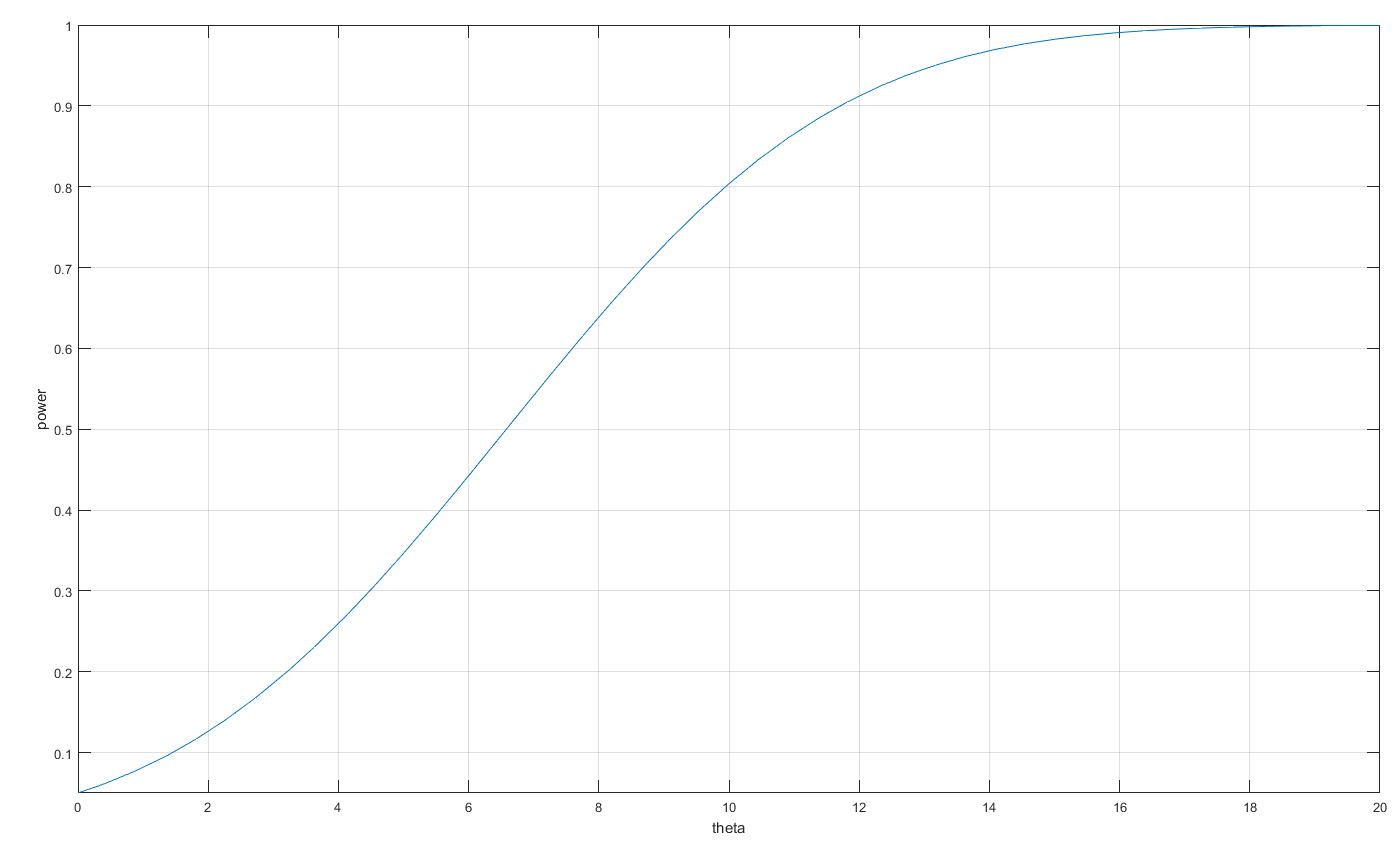
\includegraphics[width=340px]{p2c.png}
			
			\footnotesize The shape of a typical power function.
	\end{center} 
		
\end{document}
 
 	
 	